\chapter{Introduction}
\label{chap:intro}

\section{Current State of 3D Generation}

3D generative models have progressed rapidly in recent years, producing models and scenes with remarkable detail, coherence, and realism as seen in Figure \ref{fig:generated_asset}. Within the domain of digital creation, these advancements present significant opportunities for artists and designers by accelerating workflows across real-world applications such as interactive media, cinematic visual effects, and rapid prototyping. These technical advances stem primarily from innovations in neural representations like Neural Radiance Fields and 3D Gaussian Splatting, alongside the adaptation of diffusion models, and the critical release of large-scale 3D datasets such as Objaverse \cite{deitke2022objaverseuniverseannotated3d}. However, the complexity of these underlying data structures introduces a significant bottleneck. Because these models generate dense point clouds, volumetric data, or implicit surface functions rather than straightforward pixel grids, conditioning the generation process remains severely limited compared to what is possible in 2D. Users are often left with a closed generation process that yields impressive but conceptually rigid results.

\begin{figure}[H]
     \centering
     \begin{subfigure}[b]{0.30\textwidth}
         \centering
         
\includegraphics[width=\linewidth]{images/generation.png}
     \end{subfigure}
     \hspace{2cm}
     \begin{subfigure}[b]{0.30\textwidth}
         \centering
         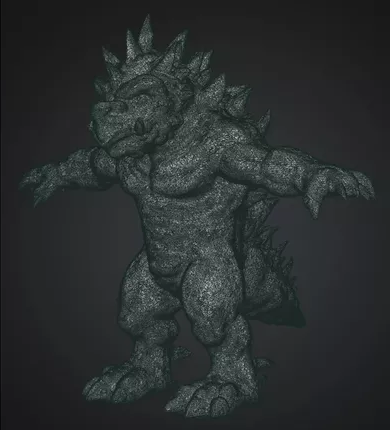
\includegraphics[width=\linewidth]{images/generation_mesh.png}
     \end{subfigure}
        \caption{Geometry and topology of a generated asset}
        \label{fig:generated_asset}
\end{figure}

In contrast, 2D generative modeling has evolved through a rich ecosystem of conditioning techniques that accommodate complex conceptualization. The relative simplicity of 2D data has enabled highly controllable diffusion frameworks that accept diverse, simultaneous forms of input. Users can guide generation using text, multiple reference images, video, bounding boxes, sketches, color palettes, depth maps, keypoints, and pose information to achieve fine-grained control over the final output \cite{Kim_2026, shi2025brickifyenablingexpressivedesign, zhang2023addingconditionalcontroltexttoimage}. This ecosystem allows creators to define the semantic, structural, and stylistic identity of an image before generation even begins. Recent work has also explored mechanisms allowing diffusion models to process and reason over these varied inputs, evaluating semantic constraints to better align with the user's overarching vision \cite{mi2025ithinkidiffuse}.

Such comprehensive conditioning techniques remain notably absent in the 3D generation space. Most current approaches rely entirely on a single text prompt or a primary reference image, occasionally supplemented by a few alternative viewing angles. While some methods incorporate alternative modalities, such as point clouds \cite{zhang20233dshape2vecset3dshaperepresentation} or sketches \cite{chen2023control3dcontrollabletextto3dgeneration}, these are isolated tools that address highly specific structural constraints. They do not offer a cohesive way to combine multiple, diverse sources of inspiration into a single generation pipeline.

Consequently, current 3D workflows struggle to translate complex artistic intent into generated assets. When a creator envisions a 3D object, the conceptualization phase rarely relies on a single sentence or a solitary image. It typically involves aggregating various visual cues, thematic references, and stylistic guidelines to form a cohesive design language. The inability of current 3D models to jointly process and harmonize a collection of diverse conditional inputs restricts their utility in professional pipelines, where nuance, composition, and multi-faceted stylistic guidance are strictly required right from the initial generation step.

\section{The Controllability Gap}

The disparity between 2D and 3D generative control stems from several fundamental challenges. First, 3D data is inherently more computationally expensive to process, requiring models to reason about geometry, topology, and appearance simultaneously across multiple viewpoints. Second, there is a distinct lack of diverse, high-quality training data for 3D content compared to the massive abundance of annotated 2D images available. Third, evaluating and iterating on 3D outputs is highly cognitively demanding; understanding spatial relationships and volumetric properties requires mental rotation and multi-perspective evaluation that 2D images do not.

This controllability gap has severe practical consequences for creative workflows. Artists and designers using current 3D generative tools are frequently trapped in a "generate-and-hope" loop, repeatedly sampling from the model until a vaguely acceptable result emerges. Unlike 2D workflows, where users can incrementally refine outputs by layering various conditioning signals, 3D generation offers very few targeted intervention points. This limitation reduces efficiency and heavily constrains creative exploration, as users cannot easily guide the model toward specific aesthetic, structural, or functional goals.

Furthermore, current 3D generation lacks the ability to disentangle and blend multiple abstract stylistic influences, a feature that is now standard in 2D workflows. For example, recent 2D interaction frameworks such as Brickify \cite{shi2025brickifyenablingexpressivedesign} allow creators to simultaneously input multiple distinct reference images to dictate texture, color palette, and structural style independently. By extracting these elements as controllable design tokens, users can blend diverse semantic concepts into a cohesive novel output, as seen in Figure \ref{fig:style-blend}.

\begin{figure}[H]
\centering
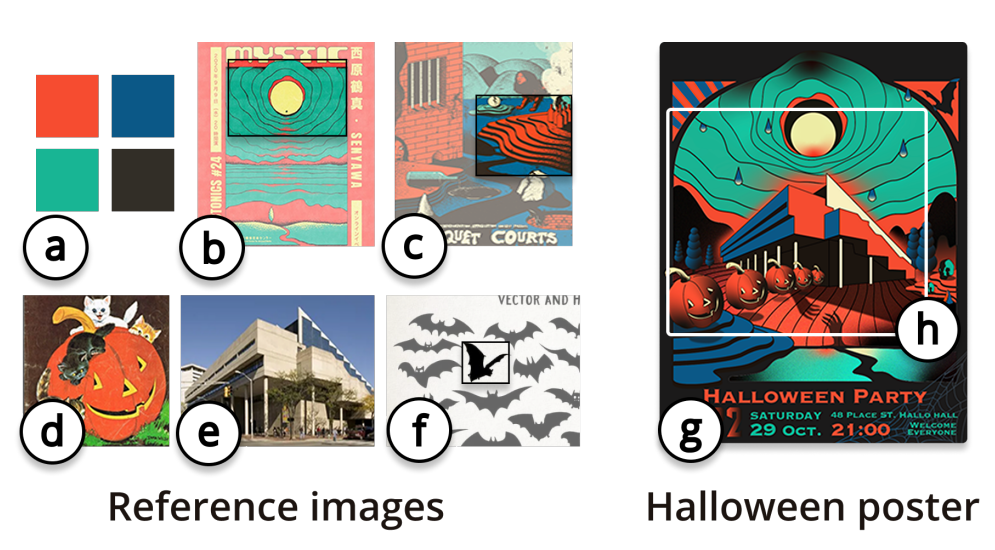
\includegraphics[width=\textwidth]{images/style-blend.png}
    \caption{Combining multiple visual references in 2D image generation.}
    \label{fig:style-blend}
\end{figure}

In contrast, when current 3D models accept multiple image inputs, they almost exclusively treat them as multi-view observations of the exact same target object for the purpose of rigid reconstruction. A 3D user cannot currently input a structural reference of a chair alongside a separate image of a rusted metal texture and expect the model to harmonize the two. They must instead rely on dense, often ambiguous text prompts. The absence of mechanisms to weight, isolate, or prioritize different visual inspirations leaves a critical gap in professional 3D pipelines, where design is inherently an act of compiling diverse references.

\section{Moodboards as a Solution}

A promising direction to bridge this controllability gap is moodboard-based input. Moodboards represent a well-established creative tool used to communicate atmosphere, style, and conceptual direction through curated arrangements of images, colors, text and more. Beyond merely aggregating visual references, moodboards allow creators to synthesize multiple distinct inspirations into a single cohesive vision. This directly addresses the limitation of current 3D models, which typically only interpret multiple image inputs as literal multi-view observations of the exact same object.

\begin{figure}[H]
\centering
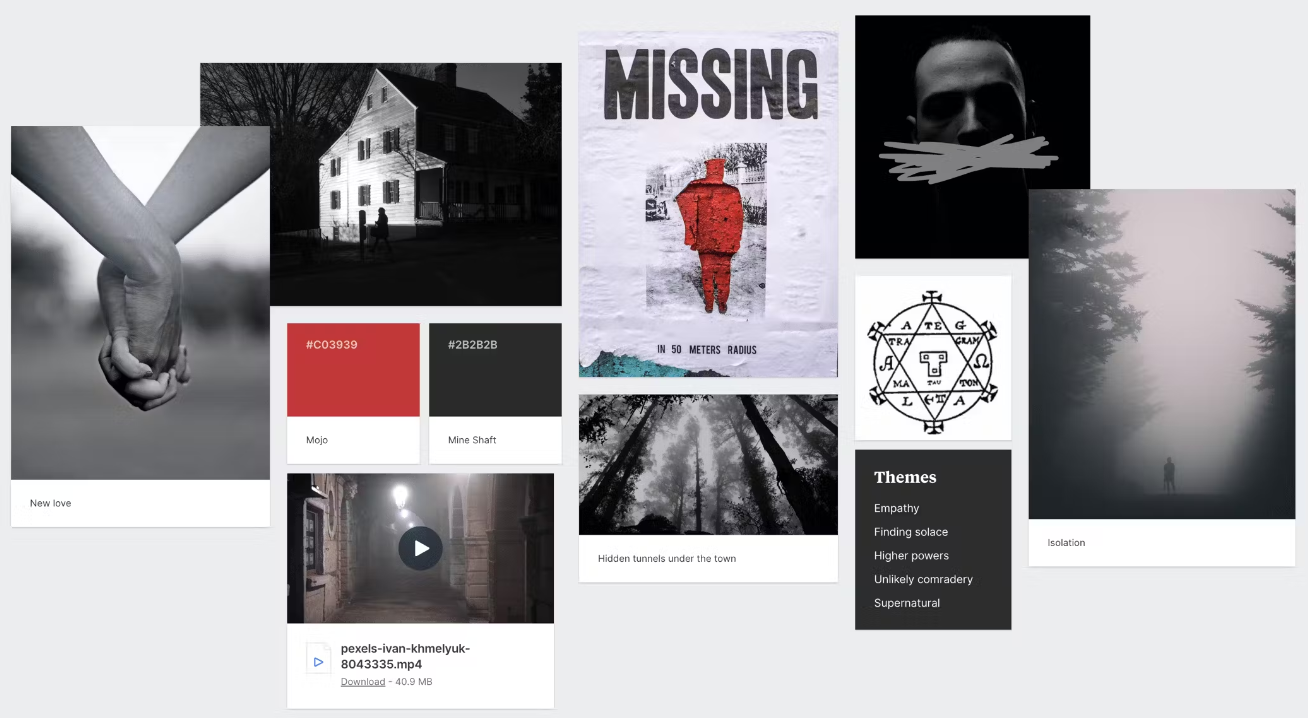
\includegraphics[width=0.8\textwidth]{images/moodboard.png}
    \caption[Moodboard example]{Example of a moodboard used in creative workflows.}
\end{figure}

The spatial arrangement of a moodboard is not arbitrary. It carries semantic weight and provides a direct mechanism for user control. Elements placed centrally or given prominence through size suggest greater importance. Clustered items indicate thematic relationships or stylistic coherence. The overall density and distribution of content communicate the balance between different influences. These implicit signals offer a powerful and intuitive control scheme that remains largely unexploited by current generative models.

Adapting this paradigm for 3D generative models offers a new way for users to interact with multiple references. Instead of relying on a closed generation process, creators gain an intuitive interface to blend distinct structural and stylistic elements. A moodboard allows a user to seamlessly combine diverse inputs, such as a base shape, a separate material reference, and a color palette. By modifying the spatial layout and directly adjusting the explicit weights of these individual elements, users can guide how the model harmonizes disparate influences into the final 3D design.

This approach expands the contextual information available to the model and integrates a familiar creative process into 3D generation workflows. Rather than encoding complex intent through ambiguous text prompts, users can leverage visual and spatial reasoning to direct the model. This guarantees that multiple diverse references can finally be utilized in a way that makes logical sense to both the designer and the generative pipeline.

\section{Research Objectives and Contributions}

By incorporating moodboard-driven interfaces, we can bridge the gap between intuitive artistic expression and technical generative modeling, enabling more natural and flexible approaches to 3D design. This dissertation explores how such systems can be developed and evaluated, with the goal of making 3D generation more accessible and expressive for creative practitioners.

A central challenge in this work is determining how moodboard layouts can be effectively encoded as conditioning signals for 3D generative models. This requires developing methods that extract both semantic content and spatial relationships from moodboard arrangements, capturing the implicit priorities and compositional structure encoded in the layout. Beyond simply aggregating reference materials, the system must understand how elements relate to one another and to the intended output.

Equally important is the question of user control and refinement. While moodboards provide rich initial context, users need mechanisms to adjust and steer the generation process based on intermediate results. We explore various approaches for enabling users to influence the model's interpretation of the moodboard, whether through iterative refinement of the layout itself, adjustment of generation parameters, or other interaction modalities that emerge from design explorations.

Evaluating the effectiveness of moodboard-based conditioning presents its own challenges. We examine how this approach compares to existing control methods in terms of output quality, alignment with user intent, and support for creative workflows. Through both quantitative metrics and qualitative assessment, we investigate whether moodboard input provides meaningful advantages over conditioning with a single text prompt and a single reference image, and under what circumstances it proves most valuable.

Finally, we consider the broader question of how moodboard-driven systems fit into iterative design processes. Rather than treating generation as a single-shot operation, we examine how users interact with these interfaces across multiple iterations, how they adjust their moodboards in response to generated outputs, and whether this approach genuinely facilitates more efficient creative exploration.

This thesis makes several key contributions to the field of controllable 3D generation. We present a novel conditioning architecture that processes moodboard layouts as structured multi-modal input while preserving the spatial relationships that give moodboards their expressive power. Through our implementation and evaluation, we develop insights into effective interaction patterns for moodboard-based control and demonstrate improved controllability compared to baseline methods. The work also provides practical considerations for integrating moodboard-driven interfaces into real-world 3D generation workflows, informed by both technical constraints and user experience principles.